\documentclass[letterpaper,12pt]{article}
\usepackage{graphicx}
\usepackage[top=1.10in,right=1.2in,bottom=1.4in,left=1.2in]{geometry} 

\frenchspacing  % Removes extra spacing after period.

\usepackage{hyperref}

\usepackage{natbib}
%\usepackage{times}

\usepackage{amsmath}
%\usepackage{hyperref}

\usepackage{color}

\usepackage{pa}

\newcommand{\proglang}{\texttt}
\newcommand{\pkg}{\texttt}


\title{EPC-interest for categorical data with an application to the Inglehart values ranking}
\date{}

\author{DL Oberski \and JK Vermunt \and G Moors
\and
Department of Methodology and Statistics\\
Tilburg University, The Netherlands}


\usepackage{bm}
\newcommand\vm[1]{% Vector or matrix
\bm{\mathrm{#1}}} 

\newcommand{\av}{\vm{a}}
\newcommand{\vech}{\mathrm{vech}\,}
\newcommand{\vecs}{\mathrm{vec}\,}
\newcommand{\param}{\vm{\theta}}
\newcommand{\bpsi}{\vm{\psi}}
\newcommand{\that}{\hat{\vm{\theta}}}
\newcommand{\psat}{\hat{\vm{\psi}}}
\newcommand{\A}{\vm{A}}
\newcommand{\g}{\vm{g}}
\newcommand{\J}{\vm{J}}
\newcommand{\Id}{\vm{I}}
\newcommand{\Ji}{\vm{J}^{-1}}
\newcommand{\PP}{\vm{P}}
\newcommand{\da}{\textrm{{\sc {EPC}}-interest}}

\usepackage{setspace}
\doublespacing

\begin{document}
\maketitle



\begin{abstract}
Social science is often concerned with comparing groups such as countries, regions, time periods, the genders, or ethnicities.
Because such substantive comparisons may be threatened when measurement parameters differ across the groups, it is common practice to test the hypothesis of exact equality of measurement parameters across groups:  ``measurement invariance testing''. However, not all measurement differences are substantively relevant. At the same time, it was recently shown that not all substantively relevant differences are necessarily detected by the current best practices of invariance testing. Therefore, it was recently suggested to detect the relevant set of violations of measurement invariance using sensitivity analysis. This approach, recently introduced in this journal, uses the ``EPC-interest'',  a measure of the change in the parameters of substantive interest due to violations of invariance. So far, however, EPC-interest was limited to continuous linear structural equation models and did not consider the impact of freeing several restrictions at the same time. 

Since categorical data are common in the social sciences and measurement invariance restrictions may be highly correlated, this paper extends the ``EPC-interest'' to models with categorical observed and latent variables. Moreover, we explicitly consider freeing (potentially large) sets of equality restrictions simultaneously. The advantages of the extended EPC-interest are demonstrated using a 48-country analysis of ``materialism / postmaterialism'' values measured by three partial ranking tasks using multilevel latent class regression. Some corroboration for hypotheses on postmaterialism from the literature are found when employing the EPC-interest, while without its application some of the findings contradict these hypotheses.

The newly developed methods discussed in this paper have been implemented in commercial software for latent variable modeling. Program inputs and data for the examples discussed in this article are provided in the electronic appendix (\url{http://}) [included as zip file in blinded version].
\end{abstract}

\section{Introduction}

\noindent

The logic of measurement invariance testing is that groups may safely be compared when their measurement parameters are exactly equal: in that case, conclusions of substantive interest are uncontaminated by measurement differences. While this logic is sound, it does not follow that comparison is never warranted when measurement parameters are not exactly equal. Moreover, in practical applications exact equality is not often plausible. These observations have led to the concept of ``approximate'' measurement  invariance, in which a certain, ``small'' amount of non-invariance is permitted. 
%``Approximate'' has in the past been taken to correspond to model fit in terms of CFI, RMSEA and other relative fit measures, while more recently Bayesian priors on group differences and the alignment method were introduced. 
However, while these methods ensure that measurement differences are ``small'', even ``small'' measurement differences could, in principle, still contaminate the conclusions of interest. Conversely, those measurement differences allowed for may not necessarily affect the conclusions of interest. 


\citep{muthen2012bayesian}
\citep{schoot2013facing}

\citep{muthen2014alignment}


\section{EPC-interest}

\begin{equation}
	\left( \frac{\partial^2 L(\param, \bpsi)}{\partial (\param, \bpsi)^\prime \partial (\param, \bpsi)} \right)^{-1}
		\left( \frac{\partial L(\param, \bpsi)}{\partial \bpsi} \right)
\end{equation}



\section{Data}

[GUY: Een mooi verhaal over Inglehart values]

[Esp. Explain why it is of interest to compare the countries on GDP/capita and \% women in parliament]

[WVS 2010--2012. $n=67^,568$ ]

[Countries: ARM AUS AZE BLR CHL CHN COL CYP DEU DZA ECU EGY ESP EST GHA IRQ JOR JPN KAZ KGZ KOR LBN LBY MAR MEX MYS NGA NLD NZL PAK PER PHL POL QAT ROU RUS RWA SGP SVN SWE TTO TUN TUR UKR URY USA UZB YEM ZWE]

Table \ref{tab:ranking-question} shows the ranking tasks asked in the WVS 2010--2012.

\begin{table}
\begin{tabular}{p{0.01\textwidth}rp{0.78\textwidth}}
\hline
& Option \# & Option wording\\
\hline
\multicolumn{3}{l}{\emph{Set A}}\\
&1. & A high level of economic growth\\
&2. & Making sure this country has strong defense forces \\
&3. & Seeing that people have more say about how things are done at their jobs and in their communities\\
&4. & Trying to make our cities and countryside more beautiful\\

\multicolumn{3}{l}{\emph{Set B}}\\
&1. & 	Maintaining order in the nation\\
&2. & Giving people more say in important government decisions \\
&3. & 	Fighting rising prices\\
&4. & Protecting freedom of speech\\

\multicolumn{3}{l}{\emph{Set C}}\\
&1. & 	A stable economy\\
&2. & Progress toward a less impersonal and more humane society \\
&3. & 	Progress toward a society in which Ideas count more than money \\
&4. & 	The fight against crime\\
\hline
	\end{tabular}
\caption{\label{tab:ranking-question}
Options to be ranked for the three Inglehart values ranking sets in 
the World Values Survey 2010--2012. The wording of the question is
``People sometimes talk about what the aims of this country should be for the next ten years. On this card are listed some of the goals which different people would give top priority. Would you please say which one of these you, yourself, consider the most important?''; ``And which would be the next most important?''.
}
\end{table}

\clearpage
\section{Model}


To examine differences in (post)materialism with respect to GDP per capita and the proportion of women in parliament, we develop a latent variable model for ranking data. The advantages of this approach are that there is no need to establish a priori rules for combining the three ranking tasks into a measure of ``postmaterialism''; that it does not presuppose a fixed number of ``postmaterialism'' classes; that it allows for measurement error in ``postmaterialism''; and that it allows for an examination of the impact of violations of measurement invariance on the conclusions of interest. 
There are several approaches to modeling ranking data. We adopt a sequential approach originally due to \citet{luce1959individual} and \citet{mcfadden1974conditional}. A single-level latent variable  version of these models was described by \citet{bockenholt2002comparison}; \citet{moors2007heterogeneity} applied a multilevel latent class model for rankings to European Values Study data on postmaterialism. Different approaches to modeling ranking data using latent variables can be found in
\citet{maydeu2005structural} and \citet{brown2011item,brown2012fitting}. 

The ranking model departs by describing the joint probability of observing choice $A_1 = a_1$ on set A (see Table \ref{tab:ranking-question}) for first place  and $A_2 = a_2$ for second place as 
\begin{equation}
	P(A_1 = a_1, A_2 = a_2 | X = x) = 
		\frac{\omega_{a_1 x}}{\sum_{k} \omega_{k x}}
		\frac{\omega_{a_2 x}}{\sum_{k \neq a_1}
			\omega_{k x}},
				\label{eq:ranking}
\end{equation}
where $\omega_{k x}$ is the utility ($0<\omega_{k x}<1$) of response option $k$ \citep{mcfadden1974conditional}. Crucially, the choice for second place, $A_2$, is modeled while excluding the alternative already chosen for first place, $A_1$. In other words, we model a sequential ranking process in which first place is chosen first, then second place is chosen from the remaining options.
This makes the model used here different from standard models for categorical data.
 The utilities $\omega_{kx}$ may differ over persons due to the latent class variable $X$ \citep[pp. 171--3]{bockenholt2002comparison}, which in our case will represent ``(post)materialism''. This latent class variable is typically chosen to have a fixed number of categories, $T$. To restrict the utilities to their allowed range and facilitate model interpretation, it is convenient instead of the utilities $\omega_{kx}$ to estimate the log-linear parameters,
\begin{equation}
	\ln \omega_{k x} = \tau_{k} + \lambda_{k x}.\label{eq:loglin-measurement}
\end{equation}
For identification, we set $\sum_k \tau_{k} = \sum_{k} \lambda_{kx} = \sum_{x} \lambda_{kx} = 0$. Using this ``effects coding''  \citep{vermunt2013technical},  the $9 (T - 1)$ attribute parameters $\lambda_{k x}$ can then be interpreted as the deviation from option $k$'s average log-utility in latent class $x$.



Primary interest focuses on how the probabilities of belonging to these latent (post)materialism classes differ as a function of the country-level covariates log-GDP per capita ($Z_1$) and percentage of women in parliament ($Z_2$).  At the same time, it has become common practice to control for country effects using a multilevel approach. We therefore model the latent class probabilities using the multinomial logistic regression
\begin{equation}
P(X = x| Z_1 = z_1, Z_2 = z_2, G = g) = \frac{\exp(\alpha_x + \gamma_{1x} z_1 +\gamma_{2x} z_2  + \beta_{gx})}
					{\sum_t \exp(\alpha_t + \gamma_{1t} z_1 +  \gamma_{2t} z_2 +  + \beta_{tg})},
					\label{eq:regression}
\end{equation}
where the country-level latent variable $G$ has been introduced. The country-level effects $\beta_{tx}$ in Equation \ref{eq:regression} could be modeled as normal, leading to a standard multilevel model. However, since in the past very differing classes of countries have been observed \citep{moors2007heterogeneity}, making the normality assumption rather implausible, we instead take $G$ to be a country-level latent class variable with $S$ classes and a freely estimated distribution. This nonparametric model was introduced as the ``multilevel latent class regression'' model by \citet{vermunt2003multilevel}. The main parameters of substantive interest in Equation \ref{eq:regression} are the $2  (T - 1)$ logistic regression coefficients $\gamma_{mx}$.


%, of which there are , where $T$ is the number of latent postmaterialism ($X$) classes. 
%It may also be of interest to derive the posterior probability for each country, $P(X | \text{country}) = \sum_{i \in \text{country}} P(Y | X) P(X) / \sum_X P(Y | X)$ for visual display purposes.

Combining the three ranking tasks, each modeled according to Equation \ref{eq:ranking}, with the multilevel latent class regression model in Equation \ref{eq:regression} leads to the casewise likelihood
\begin{multline}
L(\param) = 
	P(A_1, A_2, 
		B_1, B_2, 
		C_1, C_2 | Z_1, Z_2) = \\
	\sum_{G} P(G)	\sum_{X} P(X | Z_1, Z_2, G)
				P(A_1, A_2 | X)
				P(B_1, B_2 | X) 
				P(C_1, C_2 | X),
				\label{eq:lik}
\end{multline}
where the realizations of variables have been dropped for clarity, and $\param$ is a vector collecting the $-3 + T (11 + S) $ free parameters of the model.
Note that values of the within-country variables $X, A_1, A_2, B_1, B_2, C_1$, and $C_2$ may differ over persons, whereas the between-country variables $G, Z_1$, and $Z_2$ can differ only over countries. 


\begin{figure}\centering
	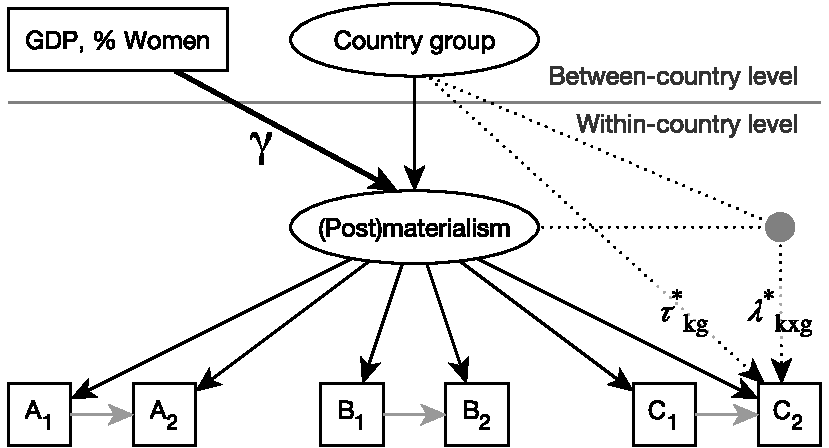
\includegraphics[width=0.7\textwidth]{figures/model}
	\caption{\label{fig:model}Graphical representation of 
	the multilevel latent class regression model for 
	(post)materialism measured by three partial ranking tasks. Observed variables are shown in rectangles while unobserved (``latent'') variables are shown in ellipses.	}
\end{figure}


Figure \ref{fig:model} shows a graphical representation of the model in Equation \ref{eq:lik}. 
The parameters of primary substantive interest are the effect-coded logistic regression coefficients for the effect of GDP per capita and percentage of women in parliament on the latent postmaterialism class (the stronger line labeled $\gamma$ in Figure \ref{fig:model}). 
These effects of interest are controlled for the country random effects. Since these are modeled using a latent class variable, the top part of the model in Figure \ref{fig:model} is a multilevel latent class regression. The gray arrows between indicators within the same set are meant to show that a fixed conditional relationship is specified between the first and second choice within each set (Equation \ref{eq:ranking}). 

Equation \ref{eq:lik} is, in fact, a full invariance model: it excludes potential violations of ``scalar''  and ``metric'' measurement invariance. These can be conceptualized as, respectively, a direct main effect and a direct interaction effect of the grouping variable 
\citep{mellenbergh1989item,kankaras2010testing,kankaras2011measurement}. Since we do not employ multiple groups (fixed effects) to deal with country effects, but a latent class multilevel (random effects) approach, instead of considering main and interaction effects from the countries directly, we consider these for the country random effects ($G$)  \citep[see][]{dejong2007relaxing,fox2011random}.
Thus, measurement invariance violations could be parameterized by extending Equation  \ref{eq:loglin-measurement} to include country group class ($g$) effects:
\begin{equation}
	\ln \omega_{k x g} = \tau_{k} + \lambda_{k x} + 
		\tau^{*}_{k g} + \lambda^{*}_{k x g}.
			\label{eq:loglin-measurement-noninvariant}
\end{equation}
The base invariance model above can then be seen as fixing the intercept deviations $\tau^{*}_{k g}$  and slope deviations $\lambda^{*}_{k x g}$ to 0.  An example of this parameterization of measurement non-invariance for 
the second ranking of Set C ($C_2$) is shown in Figure \ref{fig:model} as the dotted main effect and interaction effects for scalar and metric invariance, respectively. 

With three sets of three non-redundant ranking options each, there are $9 (S - 1) T$ possible additional $\tau^{*}_{k g}$ and $\lambda^{*}_{k x g}$ parameters representing misspecification in the full invariance model specified above. For example, with $S=3, T=3$, there will be $54$ possible violations of invariance. %With three or more second-level classes ($S \geq 3$), there are more possible violations of measurement invariance than there are parameters in the base model.
This is clearly a very large number of potential violations of measurement invariance, with an astronomical ($\approx 1.8 \times 10^{16}$) number of possible subsets of non-invariant models, making the fitting of each of these possible submodels infeasible. The EPC-interest, which considers the possible effect of freeing each of the restrictions separately, is therefore an attractive alternative. 

However, there are strong correlations between the possible additional parameters. First, parameters for different categories of the same variable will necessarily be strongly correlated. Second, parameters corresponding to the same ranking set (A, B, or C) will be highly correlated due to the necessary dependence between the first and second choice in a ranking task. Therefore, instead of considering only one possible misspecification at a time, we consider freeing sets of restrictions corresponding to all main effects and all interaction effects of each set. The advantages are that the estimated change in the parameters of interest will be closer to the observed change when freeing these restrictions, and that a model space to be explored of order $10^{16}$ is reduced to the examination of the effect of six sets of misspecifications on $2 (T-1)$  parameters of interest, $\gamma_{jx}$.

\bigskip
In summary, we have attacked the problem of examining the differences in (post)-materialism over 48 countries with different levels of GDP per capita and percentage of women in parliament by formulating a multilevel latent class model for ranking data. Measurement invariance is important here because direct main and interaction effects from country groups on the ranking tasks could threaten the comparison of countries with different levels of the covariates. Therefore it becomes relevant to examine the impact of these possible violations of measurement invariance on the parameters of substantive interest using the EPC-interest. Since the data are categorical and the possible misspecifications are highly correlated, the extensions of the EPC-interest discussed in the preceding sections become essential.


\section{Results}

Latent Gold Choice 5.0.0.14157
\citep{vermunt2005lgchoice,vermunt2013technical}

LL = -418609.9616

Number of parameters (Npar)	63

Program input can be found in Appendix \ref{sec:LGinput}, while output and data are included in the online Appendix at \url{http://}.

\begin{table}
	\begin{tabular}{lrrrrrrrrrrr}
	\hline
		&&&&&\multicolumn{7}{c}{EPC-interest for...}\\
	&&&&&\multicolumn{3}{c}{$\tau^{*}_{k g}$} && \multicolumn{3}{c}{$\lambda^{*}_{k x g}$}\\
			\hline
		&&\multicolumn{2}{c}{Estimates}&&\multicolumn{3}{c}{Ranking set} && \multicolumn{3}{c}{Ranking set}\\
\cline{3-4}\cline{6-8}\cline{10-12}
			&	&	Est.&	s.e.&	&	1  &	2  &	3  &&	  1&	2 &	3\\
				\hline
Class	1&	GDP&	-0.035&	(0.007)&	&	-0.013&	0.021&	-0.002&&	\textbf{0.073}&	\textbf{0.252}&	0.005\\
Class	2&	GDP&	-0.198&	(0.012)&	&	-0.018&	-0.035&	0.015&&	-0.163&	-0.058&	0.002\\
\\
Class	1&	Women&	0.013&	(0.001)&	&	-0.006&	0.002&	0.000&&	-0.003&	0.029&	0.002\\
Class	2&	Women&	-0.037&	(0.001)&	&	0.007&	-0.003&	0.002&&	-0.006&	-0.013&	0.002\\
	\hline
\end{tabular}
	\caption{\label{tab:epc-interest-model1}}
\end{table}

\begin{table}
	\begin{tabular}{lrrrrrrrrrrr}
	\hline
		&&&&&\multicolumn{7}{c}{EPC-interest for non-invariance of...}\\
%		&&\multicolumn{2}{c}{Estimates}&&\multicolumn{3}{c}{Set} && \multicolumn{3}{c}{Set}\\
	&&&&&\multicolumn{3}{c}{$\tau^{*}_{k g}$} && \multicolumn{3}{c}{$\lambda^{*}_{k x g}$}\\
			\hline
		&&&&&\multicolumn{3}{c}{Ranking set} && \multicolumn{3}{c}{Ranking set}\\
\cline{3-4}\cline{6-8}\cline{10-12}
			&	&	Est.&	s.e.&	&	1  &	2  &	3  &&	  1&	2 &	3\\
				\hline
Class 1&	GDP&	-0.127&	(0.008)&	&	-0.015&	-0.003&	0.002&&	&	&	0.097\\
Class 2&	GDP&	0.057&	(0.011)&	&	-0.043&	-0.013&	0.002&&	&	&	0.161\\
\\
Class 	1&	Women&	0.008&	(0.001)&	&	-0.002&	0.000&	0.002&	&&	&	0.001\\
Class 	2&	Women&	0.020&	(0.001)&	&	-0.007&	-0.001&	0.002&	&&	&	0.007\\
\hline
	\end{tabular}
	\caption{\label{tab:epc-interest-model2}}

\end{table}



\begin{table}\centering
	\begin{tabular}{llrrr}
	\hline
			&&	Class 1	&	Class 2	&	Class 3\\
			&Class label& ``Materialist'' & ``Postmater.'' & ``Mixed''\\
& Class size & 0.569 & 0.213 & 0.218\\
				\hline
\multicolumn{3}{l}{Set A}\\
& 1. Economic growth	&	2.1102	&	0.4837	&	0.4156\\
& 2. Strong defense	&	-0.5285	&	-1.4984	&	-0.9249\\
& 3. More say	&	-0.5519	&	1.4683	&	0.4643\\
& 4. More beauty	&	-1.0298	&	-0.4536	&	0.0449\\
\multicolumn{3}{l}{Set B}\\
& 1. Order in the nation	&	1.0016	&	-0.5898	&	0.0435\\
& 2. More say	&	-0.4592	&	0.6902	&	-0.2763\\
& 3. Rising prices	&	0.4281	&	-0.2269	&	0.3719\\
& 4. Freedom of speech	&	-0.9705	&	0.1266	&	-0.1390\\
\multicolumn{3}{l}{Set C}\\
& 1. Stable economy	&	2.0086	&	0.0789	&	0.1715\\
& 2. Humane society	&	-0.7919	&	0.4450	&	-0.0943\\
& 3. Ideas	&	-1.1402	&	-0.0593	&	-0.4550\\
& 4. Fight crime	&	-0.0765	&	-0.4646	&	0.3778\\
	\hline
	\end{tabular}
	\caption{\label{tab:attribute-parameters}Attribute parameter estimates for the 
		final model.}

\end{table}



\begin{figure}
	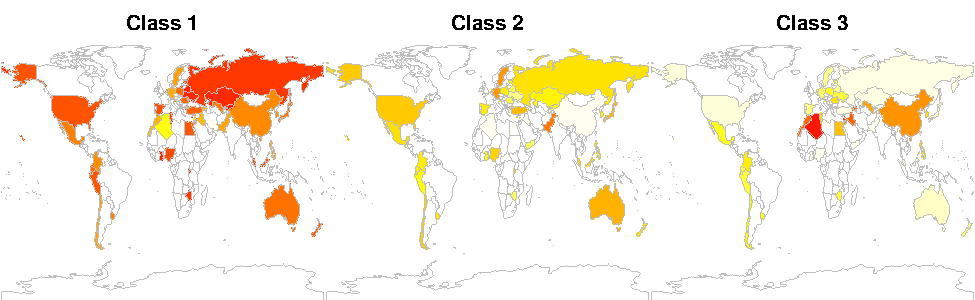
\includegraphics[width=\textwidth]{figures/maps.pdf}
	
	\caption{\label{fig:maps}}
\end{figure}

\begin{figure}
	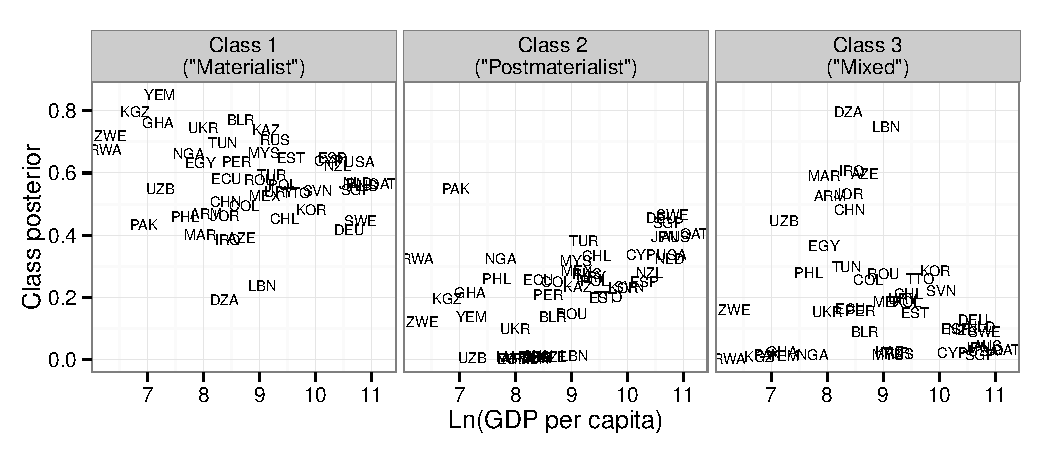
\includegraphics[width=\textwidth]{figures/gdp-posterior.pdf}
	
	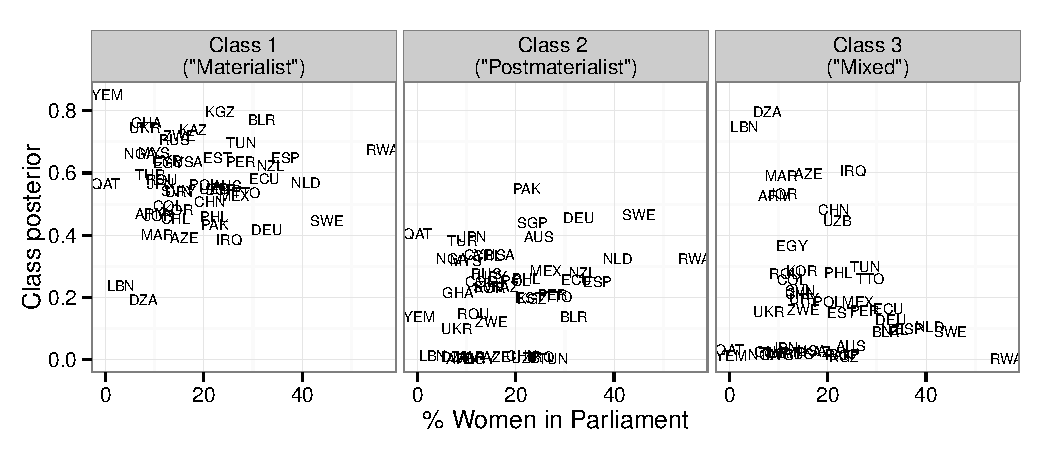
\includegraphics[width=\textwidth]{figures/women-posterior.pdf}

	\caption{\label{fig:posterior}}
\end{figure}

\begin{figure}
	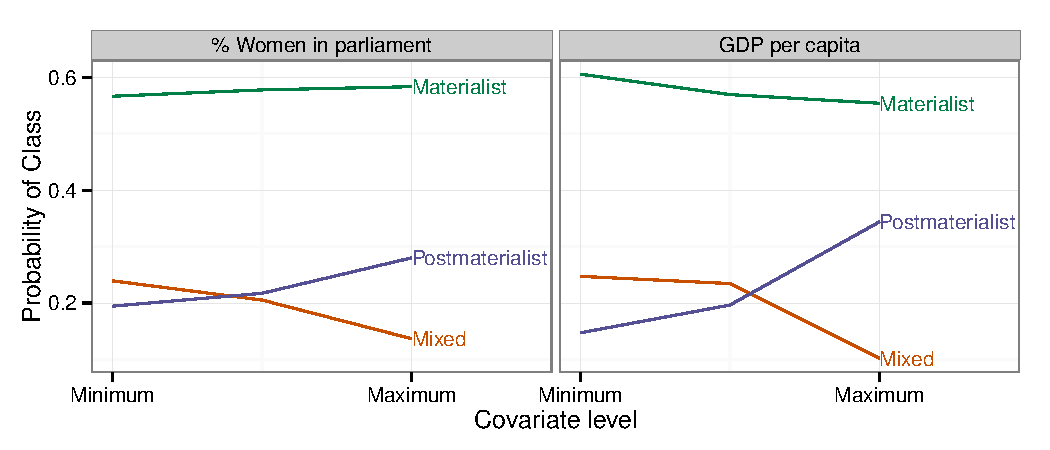
\includegraphics[width=\textwidth]{figures/covariates.pdf}
	\caption{\label{fig:covariates}Estimated probability of choosing each class as a function of the covariates of interest under the final model.}
\end{figure}


\section{Discussion}



\bibliographystyle{pa}
\bibliography{/Users/daob/Dropbox/Bibliography/quality}

\clearpage\appendix
\section{Latent Gold input for the full invariance model}\label{sec:LGinput}

The input below fits the full invariance model described in the paper, setting the possible violations of invariance to zero (0). The option ``score test'' in the output section (only available in LG $\geq5$) is then used to obtain the EPC-interest values.
Output and data for this example can be obtained from the online appendix at \url{http://}.

\begin{small}
\singlespace
\begin{verbatim}
options

   maxthreads=all;
   algorithm 
      tolerance=1e-008 emtolerance=0.01 
      emiterations=450 nriterations=70 ;
   startvalues
      seed=0 sets=30 tolerance=1e-005 iterations=50;
   bayes
      categorical=0 variances=1 latent=0 poisson=1;
   missing  excludeall;
   output      
      parameters=effect  betaopts=wl standarderrors profile 
      probmeans=posterior
      frequencies bivariateresiduals estimatedvalues=regression
      predictionstatistics setprofile setprobmeans 
      iterationdetails scoretest ;

	choice = 3
   alternatives 'inglehart_wvs6_long.alt' quote = single
   id=alt
   choicesets 'inglehart_wvs6_long.set' quote = single
   id=set;

variables
   groupid country;
   caseid id;
   choicesetid set ;
   dependent value ranking;
   independent NY_GDP_PCAP_CD, SG_GEN_PARL_ZS;
   attribute int1 nominal, int2 nominal, int3 nominal;
   latent
      GClass  group nominal 3, 
      Class nominal 3;

equations
   GClass <- 1 ;
   Class <- 1 + GClass + NY_GDP_PCAP_CD + SG_GEN_PARL_ZS;
   value <- int1 + int2 + int3 + 
      int1 Class + int2 Class + int3 Class + 
      (0) int1 GClass + (0) int2 GClass + (0) int3 GClass + 
      (0) int1 Class  GClass + 
      (0) int2 Class GClass + 
      (0) int3 Class GClass ;
\end{verbatim}

\end{small}

\end{document}
